\section{Χρόνος Παγίδευσης Διακριτού τυχαίου περιπάτου με παγίδες}
Ο σκοπός αυτού του πειράματος είναι ο υπολογισμός του χρόνου παγίδευσης ενός σωματιδίου που εκτελεί τυχαίο περίπατο, σε ένα πλέγμα με μόρια-παγίδες σε κάποιες θέσεις του. Η μεθοδολογία που θα ακολουθήσουμε σε αυτό το πείραμα διαφέρει κατά πολύ από αυτές των προηγούμενων πειραμάτων κυρίως λόγω της δομής του κώδικα. Για την καλύτερη δόμηση και την επίτευξη γενικότητας στον κώδικα, θα χρησιμοποιηθεί αντικειμενοστραφής προγραμματισμός. Θα δημιουργήσουμε μία κλάση ονόματι {\en \texttt{grid\_2D}} όπου θα έχει όλες τις ιδιότητες που χρειάζονται για την εκτέλεση του τυχαίου περιπάτου με παγίδες. Ενώ εξηγούμε την δομή του κώδικα και τις λεπτομέρειες των εντολών, θα αναδύεται και η μοντελοποίηση του προβλήματος από υπολογιστικής σκοπιάς.

Ξεκινάμε λοιπόν με την {\en magic method \texttt{\_\_init\_\_}} που εκτελείτε με το που δημιουργείτε το αντικείμενο (κάποιο {\en instance}) αυτής της κλάσης.
\en 
\begin{python}
def __init__( self, x , y):
    self.x = x
    self.y = y
    self.grid = np.zeros((x,y),dtype=int)
\end{python}
\gr 
Δημιουργούμε ένα αντικείμενο της κλάσης {\en \texttt{grid\_2D}} δίνοντας τις διαστάσεις ενός πίνακα ({\en np.array}) τον οποίο γεμίζουμε με μηδενικά. Αυτό είναι το δισδιάστατο πλέγμα μας $x$ γραμμών και $y$ στηλών μοντελοποιημένο σε ένα πίνακα $x \times y$. 

Η επόμενη μέθοδος που θα εντάξουμε στην κλάση μας είναι για την προσθήκη παγίδων-μορίων συγκεκριμένης συγκέντρωσης:
\en 
\begin{python}
N = int((self.x*self.y)*c)
molecules = 0
while molecules<N:
    x = random.randint(0,self.x-1)
    y = random.randint(0,self.y-1)
    if self.grid[x,y]==0:
        self.grid[x,y]=1
        molecules+=1
\end{python}
\gr
Για να γεμίσουμε με κατάλληλο τρόπο το πλέγμα βρίσκουμε πρώτα τον αριθμό των παγίδων που πρέπει να τοποθετήσουμε με βάση τη συγκέντρωση \eqref{conc}. Συνεπώς, $Ν=xyc$  θα είναι ο αριθμός των παγίδων που πρέπει να τοποθετήσουμε στο {\en grid} προκειμένου να έχει συγκέντρωση $c$. Στην συνέχεια, ξεκινάμε να τοποθετούμε τον αριθμό 1(παγίδες) σε θέσεις του πλέγματος που έχουν 0 μέχρι να τοποθετηθούν και τα $N$ παγίδες-μόρια. Στο τέλος έχουμε στην κατοχή μας έναν πίνακα με $Ν$ άσσους-παγίδες και $xy-N$ ελεύθερες θέσεις για τον τυχαίο περίπατο.

Η επόμενη μέθοδος της κλάσης μας επιλέγει μία κενή θέση του πλέγματος τυχαία για την αρχική θέση του σωματιδίου και την εκκίνηση του τυχαίου περιπάτου. 
\newpage
\noindent
Ο κώδικας: 
\en
\begin{python}
def add_particle(self):
    while True:
        x = random.randint(0,self.x-1)
        y = random.randint(0,self.y-1)
        if self.grid[x,y]==0:
            self.particle_position = [x,y]
            break
\end{python}
\gr 
Έχουμε δηλαδή μία αυθαίρετη επανάληψη όπου επιλέγει τυχαία θέσεις του πλέγματος μέχρι να βρει κάποια κενή. Όταν βρει κενή θέση σταματάει η επανάληψη και αποθηκεύει την τοποθεσία του πλέγματος ως αρχική θέση του σωματιδίου.

Η επόμενη μέθοδος της κλάσης μας θα είναι η εκτέλεση του τυχαίου περιπάτου. Για να το κάνουμε αυτό αρχικά ας δημιουργήσουμε με ξεχωριστή συνάρτηση η οποία θα επιστρέφει την νέα θέση του σωματιδίου. Ο λόγος για να δημιουργηθεί μία τέτοια συνάρτηση ανεξάρτητα από το υπόλοιπο πρόβλημα, είναι η συνοριακές συνθήκες που θέλουμε να θέσουμε στο πλέγμα. Στην προκειμένη περίπτωση, όταν το σωματίδιο βρίσκεται σε μία θέση στην άκρη του πλέγματος και κινηθεί προς την κατεύθυνση που δεν υπάρχει άλλη θέση στο πλέγμα, τότε πρέπει να βρεθεί στην απέναντι πλευρά. Δηλαδή, η απέναντι πλευρές του πλέγματος λειτουργούν ως επιφάνεια κυλίνδρου. Παράδειγμα, αν έχω ένα πλέγμα 3{\en x}3, το σωματίδιο βρίσκεται στην θέση [0,0] και η τυχαία επιλογή βήματος δώσει {\en up}, η νέα θέση θα είναι η [2,0]. Αν η τυχαία επιλογή δώσει {\en left} τότε η νέα θέση πρέπει να είναι η [0,2]. Για να πετύχουμε την παραπάνω συμπεριφορά και τις κατάλληλες θεωρητικές εκμεταλλευόμαστε την συνάρτηση {\en mod} ως εξής:
\en
\begin{python}
def get_next_position(pos,rows,columns):
    move = random.choice(['left','right','up','down'])
    if move=='left':
        return [pos[0],(pos[1]-1)%columns]
    elif move=='right':
        return [pos[0],(pos[1]+1)%columns]
    elif move=='up':
        return [(pos[0]-1)%rows, pos[1]]
    elif move=='down':
        return [(pos[0]+1)%rows, pos[1]]
\end{python}
\gr 
Η συνάρτηση δέχεται ως είσοδο την προηγούμενη θέση του σωματιδίου και τις διαστάσεις του πλέγματος,  προκειμένου να γνωρίζει πότε βρίσκεται σε ακριανή θέση, καθώς και πως να ανανεώσει και να επιστρέψει τη νέα θέση. 
\newpage
\noindent
Ο τυχαίος περίπατος :
\en 
\begin{python}
def random_walk(self):
    position = self.particle_position
    steps=0
    while True:
        next_position = get_next_position(position,self.x,self.y)
        if self.grid[next_position[0],next_position[1]]==1:
            steps+=1
            break
        else:
            position = next_position
            steps+=1
    return steps
\end{python}
\gr 
Έχουμε λοιπόν το σωματίδιο σε μία τυχαία επιλεγμένη θέση και ξεκινάει τον τυχαίο περίπατο μέχρι να συναντήσει μία παγίδα. Μόλις βρεθεί στην παγίδα, επιστρέφει τον αριθμό των βημάτων που έκανε το σωματίδιο. Αυτό ήταν και το ζητούμενο, δηλαδή ο χρόνος παγίδευσης.

\gr 
Για να εκτελέσουμε λοιπόν ένα πείραμα τυχαίου περιπάτου θα πρέπει να δημιουργήσουμε το {\en grid}, να προσθέσουμε τις παγίδες, να επιλέξουμε αρχική θέση για το σωματίδιο, και να εκτελέσουμε τον τυχαίο περίπατο. Ο αλγόριθμος μοναδικού πειράματος έχεις ως εξής:
\en
\begin{lstlisting}
//=============================================================//
create grid
add molecule_traps
add particle
do the random walk - get trap_times
//=============================================================//
\end{lstlisting}
\gr 
\subsection{Πλέγμα 500{\en x}500 - Συγκέντρωση παγίδων {\en c}=0.01}
Πάμε τώρα να χρησιμοποιήσουμε τις μεθόδους αυτές για να εκτελέσουμε το πείραμα. Ας δημιουργήσουμε το πλέγμα 500{\en x}500 ως {\en instance} της κλάσης μας, και ας τοποθετήσουμε και τις παγίδες με συγκέντρωση 0.01:
\en 
\begin{python}
c = 0.01
grid1 = grid_2D(500,500)
grid1.add_molecule_traps(c)
\end{python}
\gr 
Στη συνεχεία θα πρέπει να εκτελέσουμε σε αυτό το πλέγμα 100000 πειράματα και να αποθηκεύσουμε του χρόνους διαφυγής.
\en
\begin{python}
start_time = time.time()

trap_times1 = []
for i in range(100000):
    grid1.add_particle()
    trap_times1.append(grid1.random_walk())

data1 = trap_times1.copy()
print(f"Execution time: {(time.time() - start_time)} seconds")
\end{python}
\gr 
με {\en Execution time: 25.733628273010254 seconds}. 

Έχοντας τώρα ένα μεγάλο δείγμα των χρόνων παγίδευσης μπορούμε να σχεδιάσουμε την κατανομή τους. Δύο τρόποι μπορούν να περιγράψουν την αριθμητική κατανομή των χρόνων παγίδευσης, το ιστόγραμμα και το γράφημα της κατανομής. 
Για το ιστόγραμμα χρησιμοποιούμε το πακέτο {\en matplotlib.pyplot} με το ακρωνύμιο {\en plt}:
\en 
\begin{python}
plt.hist(data1, bins = 100, color = 'blue')
plt.grid(color='0.25', linestyle='--', linewidth=0.2)
plt.ylabel('Number of Occurrences')
plt.xlabel('Trap times')
plt.title('Trap Times Histogram | 500x500 grid | c=0.01')
plt.show()
\end{python}
\gr και το γράφημα:
\begin{figure}[H]
\begin{center}
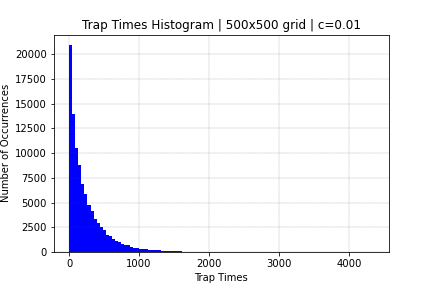
\includegraphics[scale=0.7]{figures/TRW_001_hist.png}
\caption{Ιστόγραμμα αριθμητικών περιστατικών ανά χρόνο διαφυγής για πλέγμα 500{\en x}500 με πυκνότητα παγίδων {\en c}=0.01}
\label{figuridion3d}
\end{center}
\end{figure}

Για την κατανομή πυκνότητας των χρόνων διαφυγής θα χρησιμοποιήσουμε το πακέτο {\en seaborn} με το ακρωνύμιο {\en sns}:
\en 
\begin{python}
sns.displot(data1, kind="kde", color = "blue")
plt.grid(color='0.25', linestyle='--', linewidth=0.2)
plt.ylabel('Trap Times Density')
plt.xlabel('Trap Times')
plt.title('Trap Times Density Distribution | 500x500 grid | c=0.01')
plt.tight_layout()
plt.show()
\end{python}
\gr και το γράφημα:
\begin{figure}[H]
\begin{center}
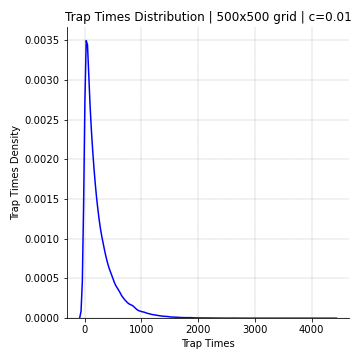
\includegraphics[scale=0.7]{figures/TRW_001_dens.png}
\caption{Κατανομή πυκνότητας χρόνων διαφυγής για πλέγμα 500{\en x}500 με πυκνότητα παγίδων {\en c}=0.01}
\label{figuridion3d}
\end{center}
\end{figure}
\subsection{Πλέγμα 500{\en x}500 - Συγκέντρωση παγίδων {\en c}=0.001}
Όμοια με προηγουμένως, με την μόνη τροποποίηση την αλλαγή της συγκέντρωσης. Δημιουργούμε το πλέγμα:
\en 
\begin{python}
c = 0.01
grid1 = grid_2D(500,500)
grid1.add_molecule_traps(c)
\end{python}
\gr 
Στη συνεχεία θα πρέπει να εκτελέσουμε σε αυτό το πλέγμα 100000 πειράματα και να αποθηκεύσουμε του χρόνους διαφυγής.
\en
\begin{python}
start_time = time.time()

trap_times2 = [] 
for i in range(100000):
    grid2.add_particle()
    trap_times2.append(grid2.random_walk())

data2 = trap_times2.copy()
print(f"Execution time: {(time.time() - start_time)} seconds")
\end{python}
\gr 
με {\en Execution time: 337.0471861362457 seconds}. 
\noindent
Το ιστόγραμμα:
\en 
\begin{python}
plt.hist(data2, bins = 100, color = 'orange')
plt.grid(color='0.25', linestyle='--', linewidth=0.2)
plt.ylabel('Number of Occurrences')
plt.xlabel('Trap Times')
plt.title('Trap Times Histogram | 500x500 grid | c=0.001')
plt.show()
\end{python}
\gr και το γράφημα:
\begin{figure}[H]
\begin{center}
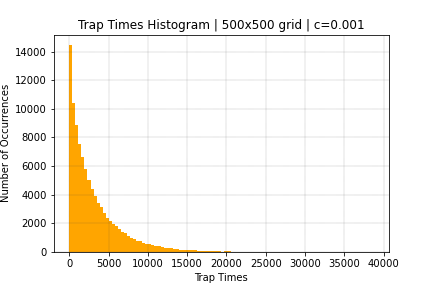
\includegraphics[scale=0.9]{figures/TRW_0001_hist.png}
\caption{Ιστόγραμμα αριθμητικών περιστατικών ανά χρόνο διαφυγής για πλέγμα 500{\en x}500 με πυκνότητα παγίδων {\en c}=0.001}
\end{center}
\end{figure}
\newpage
\noindent
Για την κατανομή πυκνότητας των χρόνων διαφυγής:
\en 
\begin{python}
sns.displot(data2, kind="kde", color = "orange")
plt.grid(color='0.25', linestyle='--', linewidth=0.2)
plt.locator_params(axis='x', nbins=5)
plt.ylabel('Trap Times Density')
plt.xlabel('Trap Times')
plt.title('Trap Times Density Distribution | 500x500 grid | c=0.001')
plt.tight_layout()
plt.show()
\end{python}
\gr και το γράφημα:
\begin{figure}[H]
\begin{center}
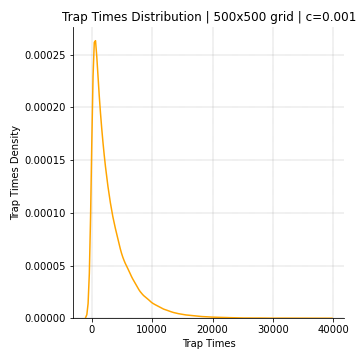
\includegraphics[scale=0.7]{figures/TRW_0001_dens.png}
\caption{Κατανομή πυκνότητας χρόνων διαφυγής για πλέγμα 500{\en x}500 με πυκνότητα παγίδων {\en c}=0.001}
\label{figuridion3d}
\end{center}
\end{figure}
\subsection{Σύγκριση των συγκεντρώσεων 0.01 και 0.001}
Τοποθετούμε λοιπόν τα δύο διαγράμματα πυκνότητας στο ίδιο διάγραμμα ώστε να παρατηρήσουμε καλύτερα την μεγάλη διαφορά που έχουν. Για να το κάνουμε αυτό εξάγουμε τα δεδομένα της γραμμής των εντολών {\en displot} που δημιούργησαν τα διαγράμματα πυκνότητας:
\en
\begin{python}
(line1_x, line1_y) = sns.distplot(data1).get_lines()[0].get_data()
(line2_x, line2_y) = sns.distplot(data2).get_lines()[0].get_data()
\end{python}
\gr 
και τα χρησιμοποιούμε για να σχεδιάσουμε μαζί τις γραμμές:
\en
\begin{python}
plt.plot(line1_x, line1_y, color='blue', label = '0.01')
plt.plot(line2_x, line2_y, color='orange', label = '0.001')
plt.xlim(0,5000)
plt.grid(color='0.25', linestyle='--', linewidth=0.2)
plt.ylabel('Trap Times Density')
plt.xlabel('Trap Times')
plt.title('Trap Times Densities | 500x500 grid |')
plt.tight_layout()
plt.legend()
plt.show()
\end{python}
\gr 
και το γράφημα:
\begin{figure}[H]
\begin{center}
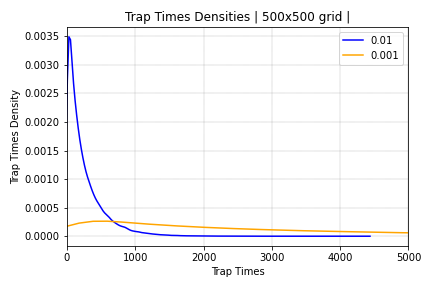
\includegraphics[scale=1]{figures/TRW_both_dist.png}
\caption{Κατανομή πυκνότητας χρόνων διαφυγής για πλέγμα 500{\en x}500 με πυκνότητα παγίδων {\en c}=0.01 και {\en c}=0.001.}
\label{figuridion3d}
\end{center}
\end{figure}

Το διάγραμμα αυτό σχεδιάστηκε έμμεσα καθώς εξάγαμε τιμές μιας αριθμητικής προσέγγισης της κατανομής των χρόνων παγίδευσης. Γι' αυτό και μερικές φορές σε αυτά τα διαγράμματα παρατηρούμε μικρές παρεκκλίσεις από αυτό που θα περιμέναμε. Για παράδειγμα βλέπουμε τα {\en displot} στην αρχή του άξονα να μοιάζουν σαν να παίρνουν αρνητικές τιμές. Προφανώς είναι αδύνατο να υπάρξει αρνητικός χρόνος διαφυγής. Αυτό συμβαίνει γιατί η βιβλιοθήκη {\en matplotlib} κάνει {\en fitting} τα δεδομένα σε συγκεκριμένες κατανομές φιξάροντας της παραμέτρους ώστε να αναπαράγουν τα δεδομένα μας. Αποτέλεσμα αυτού, μερικές φορές να υπάρχει μικρές αποκλίσεις από τα πραγματικά νούμερα. Πρόκειται δηλαδή για καθαρά υπολογιστικό λάθος και όχι για κάτι με φυσική φαινομενολογία.
\subsection{Πειραματική επιβεβαίωση της προσέγγισης {\en Rosenstock}}
\label{rosen}
Τελευταίο βήμα στη μελέτη των χρόνων διαφυγής αποτελεί η σύγκριση με την θεωρητική προσέγγιση {\en Rosenstock} για να ελέγξουμε πειραματικά την εγκυρότητά της. Σχεδιάζουμε λοιπόν σε κοινό διάγραμμα για τις δύο διαφορετικές συγκεντρώσεις την πειραματική τιμή που υπολογίσαμε παραπάνω, και την καμπύλη που προκύπτει από την {\en Rosenstock} για δύο διαστάσεις.
\noindent
Για συγκέντρωση {\en c=0.01} ο κώδικας:
\en 
\begin{python}
n = np.arange(1,5000,1)
s_n = [(1-0.01)**((np.pi*n)/np.log(n)) for n in n]
norm_const1 = np.sum(s_n)
s_n = [x/norm_const1 for x in s_n]

sns.displot(data1, kind="kde", color = "blue", label = 'Experimental')
plt.plot(n,s_n,color='black',label = 'Rosenstock')
plt.xlim(0,2000)
plt.grid(color='0.25', linestyle='--', linewidth=0.2)
plt.ylabel('Trap Times Density')
plt.xlabel('Trap Times')
plt.title('Experimental Data vs Rosenstock Data|c=0.01')
plt.legend()
plt.tight_layout()
plt.show()
\end{python}
\gr 
όπου στο πρώτο κομμάτι του κώδικα κατασκευάζουμε τις τετμημένες ({\en \texttt{s\_n}}) και τις τεταγμένες ({\en \texttt{n}}) της θεωρητικής προσέγγισης, κανονικοποιώντας την κατανομή {\en \texttt{s\_n}} για να είναι συμβατή με την κανονικοποίηση του {\en displot} και την φόρμουλα \eqref{norm}.
\newpage
\noindent
Το {\en output}:
\begin{figure}[H]
\begin{center}
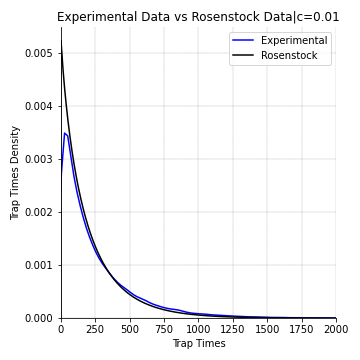
\includegraphics[scale=0.7]{figures/Rosenstock_001.png}
\end{center}
\end{figure}
\noindent
Ομοίως για συγκέντρωση {\en c=0.001}:
\en 
\begin{python}
n = np.arange(1,30000,1)
s_n = [(1-0.001)**((np.pi*n)/np.log(n)) for n in n]
norm_const1 = np.sum(s_n)
s_n = [x/norm_const1 for x in s_n]

sns.displot(data2, kind="kde", color = "blue", label = 'Experimental')
plt.plot(n,s_n,color='black',label = 'Rosenstock')
plt.xlim(0,15000)
plt.grid(color='0.25', linestyle='--', linewidth=0.2)
plt.ylabel('Trap Times Density')
plt.xlabel('Trap Times')
plt.title('Experimental Data vs Rosenstock Data|c=0.01')
plt.legend()
plt.tight_layout()
plt.show()
\end{python}
\gr 
\newpage
\noindent
Το {\en output}:
\begin{figure}[H]
\begin{center}
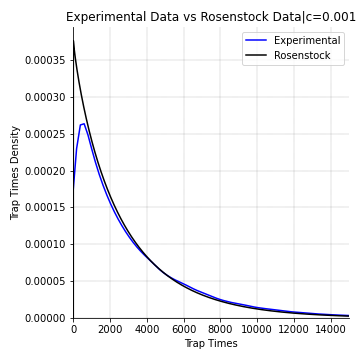
\includegraphics[scale=1]{figures/Rosenstock_0001.png}
\end{center}
\end{figure}